\chapter*{Making Sense of Systems Thinking}
\addcontentsline{toc}{chapter}{transform} 

\openepigraph{%
Managers are not confronted with problems that are independent of each other, but with dynamic situations that consist of complex systems of changing problems that interact with each other. I call such situations messes. Problems are extracted from messes by analysis. Managers do not solve problems, they manage messes.
}{Russell Ackoff}

\marginnote{
	\newthought{Key Takeaway:} Public Health Intelligence provides information to decision-makers and then... 'job done'. We need to know why they keep coming back to us with variations on the same questions, year after year. Problems don't stay solved.
}

I've been developing my systems practice for years, and I still have questions. All the time. If like me, you ask yourself questions as a way to focus, then perhaps you can relate to at least some of the following questions.

\begin{quotation}
Why all of a sudden is everybody interested in systems?

Why all of a sudden has quality become a big thing?

Why all of a sudden 'organisational learning'?

Or process re-engineering? Why?

These things, if you start reflecting on them, have been around for a long time. There have always been consumers with expectations. 

Why didn't we worry about quality before?

There have always been systems. Why?
\end{quotation}

These aren't my questions though. They are the opening words of a seminal lecture by the late great systems thinker, Russel Ackoff.\cite{Ackoff93}


\newthought{What next for Public Health?} In the last chapter, I set out where we are now, how we got into our current state and why we can't go much further. The solution seems obvious to me, but I've been thinking about this for a while now. It's not a new idea, it's not even new to public health. However, the practice of a systems-based public health will still take years yet to take root in a meaningful way.

Systems-based practice has been aptly demonstrated in the military and car manufacturing industry. kjdfkj dfkjf lfkj jfjf lkjdlfkfjlfj flkjfjf fflf. In both cases the impact was nothing short of transformational.

However, you've probably had a look at systems thinking at some point, maybe read a book or academic paper or two, right? Maybe you've heard other people talking about systems thinking, perhaps even demonstrating its use in some area of public health? I've done all of the above and more. For years I thought I could see glimpses of what it had to offer; I could get my head around some of the basic concepts, particularly those offered in systems dynamics. Then I would get stuck, distracted, I could never move my thinking on. I even started this book a couple years ago and then it languished, because I couldn't see 'the big picture' quite clearly enough to try and articulate it, which means I didn't understand it nearly well enough anyway!

Maybe you and I got to similar 'so what' stages of our learning. I think my breakthrough came from a combination of things: wider reading, a short course on critical systems thinking, the Covid19 pandemic, a couple career opportunities where I was given the scope to experiment, and maybe just more than a little frustration with public health intelligence and public health practice in general.

There were a lot of epiphanies along the way, as there should be in learning, but the big revelation (so far) isn't that we have to discard the current practice of public health intelligence or that the practice of public health more widely needs a radical course correction. There need be no root and branch rethinking of the public health discipline. Whew.

Systems-based public health practice will be transformational, of that I am convinced, and the changes to the way our organisations think, do and learn will be profound. However, in a couple decades from now (change is never quick, but we are moving), new entrants into public health practice will probably be asking what all the fuss was about. Systems-based practice will just seem like a sensible natural evolution of public health.

So what do we have to do in order to reap all these benefits? First, public health has to accept that it isn't going to 'solve' public health problems any more. We will not be eradicating any diseases (although that may happen), as we did with smallpox; problems will never again 'stay solved', as they seem to have with drinking water pathogens in developed urban environments. Second, public health intelligence will have to accept responsibility for more than counting deaths and making cool graphs so that other people understand what is happening. We have to be at least as interested in 'why' they are happening and (this is going to be painful) 'why people think' the events are happening.

Systems-based public health practice will require us to focus on managing dynamic systems and to understand how and why the patterns of population health are arising, so that we can adjust our management accordingly. When we do this, we will have nothing short of transformational impacts on health and wellbeing.

%\section*{What do we need to know}
%\begin{enumerate}
%\item What can synthesis add to analysis?
%\item Where has come from and why isn't everyone using it!
%\item Systems Thinking in Public Health
%\end{enumerate}

%(Figure~\ref{fig:navdiag2}).
%
%\begin{marginfigure}[6 cm]%
% \includegraphics[width=3cm]{./figures/NavDiag2.png}
% \centering
%  \bigskip
%  \caption{This is a place holder for a margin figure for a visual process graphic that will develop over the course of the book.}
%  \label{fig:navdiag2}
%\end{marginfigure}
\section{The long and winding road into a relevant systems thinking mindset}
%\section{What makes a good 'systems thinking' practice?}
%\section{A false start, a blind alley and then Russell Ackoff}
\subsection{A false start and a blind alley}
What do you know about systems thinking? If you are starting where I, and many others, started, you probably heard that systems thinking is about relationships, feedback loops, leverage points, and system archetypes. These aren't wrong, but they can skew your view of what systems thinking is all about. This is more formally known as the field of System Dynamics, and is where I started learning about 'systems thinking'. I blame Senge\cite{senge2010fifth} and Meadows\cite{meadows2008thinking} and their wonderfully engaging writing!

Senge and Meadows brought System Dynamics to new audiences and their books were, and still are, wildly popular. They still resonate with both my scientific and public health training and experience. However, in retrospect System Dynamics was a bit of a false start for me. In trying to understand how to use systems thinking in my public health intelligence role, System Dynamics immediately became the shining light. A light so bright that I could only 'see' systems and Systems Thinking from a Systems Dynamics perspective (Table:\ref{tab:sysdyndfn}).

\begin{table}[h]
	\begin{center}
		\footnotesize%
		\begin{tabular}{p{1.75cm} p{3.75cm} p{3.75cm}}
			\toprule
			 & System & Systems Thinking \\
			\midrule
			Senge    & "A system is a set of interrelated parts that together form a whole." & "The discipline of working with the relationships between the parts to help us see how things that may appear as separate 'parts' are actually parts of a larger pattern." \\
			\midrule
			Meadows & "A system is an interconnected set of elements that is coherently organized in a way that achieves something... a system must consist of three kinds of things: elements, interconnections, and a function or purpose." & Systems thinking is seeing interrelationships rather than linear cause-effect chains, and of seeing processes of change rather than snapshots *. \linebreak \linebreak * This is not a quote; it's my interpretation. \\
			\bottomrule
		\end{tabular}
	\end{center}
	\caption{Definitions offered by Senge and Meadows, two popular proponents of Systems Thinking, from a System Dynamics perspective.}
	\label{tab:sysdyndfn}
\end{table}

Lest I be mistaken as being critical of either of these fabulous authors or indeed of the field of System Dynamics, let me categorically state that that isn't my intention. On the contrary, System Dynamics, as I hope you will see later is central to many of our health 'system' problems for reasons I will explain in this chapter.

Getting sucked into System Dynamics, especially simulation modelling, has been one of the most interesting and useful skills I've ever picked up. However, having a really good 'hammer' maybe even a 'magic hammer' usually means that you spend a long time looking for nails. Not every problem is a nail. Nonetheless, it can be an incredibly powerful approach to understanding some types of systems (cf. see some of the case studies in the appendices). The key point to make at this point is that you'll probably be struggling to connect the field of Systems Dynamics to your work in public health (excepting obvious disease process applications like Covid19), at least at a conceptual level.

\subsection{The revelation that is Russell Ackoff!} 
It was a complete accident that I stumbled upon Ackoff's work. None of my System Dynamics reading led me to his work. I just happened to put 'systems thinking' into YouTube.com. I had never done that before, as I don't naturally turn to video for learning (or at least I didn't), I used to get all my information from reading. Not any more! I stumbled upon many systems thinking videos, most of them from the System Dynamics paradigm. Some were cute and clever, some were long and boring (academics take note!).

And then I found an Ackoff video. Smart, engaging, storytelling like I had never really encountered before. At least not in an educational orientation. I couldn't find much in the way of his writing so I kept hunting for videos on YouTube. Oh my. He gave a lot of speeches, many of which were videotaped in the 1990s through to his death in 2009. I've found about 40 hours of Ackoff on YouTube.

\begin{itemize}
	\item US Navy, 2-day workshop, 8 videos
	\item Thinking in Action Conference, From Mechanistic to Systemic Thinking, 1993
	\item Systems Thinking, Learning, and Problem Solving
	\item Annual Ackoff Lecture Series, Deming Cooperative (2003-2006), 24 videos
	\item Bell Labs (maybe), Systems Lecture
	\item University of Cincinnati, Systems-Based Improvement, 4 videos, 1995
\end{itemize}

There are many more videos of his talks, but most are small segments of the talks listed above. There are a few interviews though that are interesting, but they don't reveal much more. Furthermore, if you watch a significant number of the above videos you can see some of his ideas and stories evolve.

\subsection{Systems Thinking According to Ackoff}

Is it about looking at the interconnectedness of things? Or is it about appreciating that system behaviour (and outcomes) is dependent upon the interrelationships between parts? Many writers have used the phrase "more than just the sum of the parts" to characterise system outcomes. Ackoff when as far as suggesting that system outcomes were more like the product of the interrelationships between parts. Ackoff wasn't trying to make a serious mathematical point, he was just trying to emphasise the importance of relationships in defining how systems behave\cite{AckoffXXtbd}.

One of the key aspects of a system thinking approach was defined by Russell Ackoff as three step synthesis process (Table~\ref{tab:synthesis}). As we'll see in later sections, this leads the system practitioner towards a level of understanding best characterised as an explanation of why we have the current problem. Perhaps we are focussed on reducing cardiovascular (CVD) deaths in our community. A not uncommon public health focus. First we look to explore what these deaths a part of, i.e. what might be the containing system?

\begin{table}[h]
	\begin{center}
		\footnotesize%
		\begin{tabular}{p{4cm} p{5cm}}
			\toprule
			Process & Example  \\
			\midrule
			Step 1: What is this a part of? & CVD deaths represent one component of a population health\\
			Step 2: Understand the containing system & An Integrated Care System might be the containing whole of interest\\
			Step 3: Disaggregate the system into its controlling parts & Elements of interest might include treatment, waiting times for treatment, access to treatment, understanding of treatment options\\
			\bottomrule
		\end{tabular}
	\end{center}
	\caption{Russell Ackoff's three step process defining synthesis.}
	\label{tab:synthesis}
\end{table}

This is in contrast to our current approach, analysis thinking, that takes us down the path of breaking this problem up into component parts, which develops knowledge about the problem (Table~\ref{tab:analysisthinking}). Synthesis doesn't take us down that pathway, instead it leads us towards an explanation of why, for example, we have a problem with CVD deaths. Furthermore, and perhaps more importantly, Ackoff is giving us a 'problem solving' definition of systems thinking that resonates with purpose of public health intelligence and the wider discipline of public health (Figure~\ref{fig:stda}).

\begin{figure}
	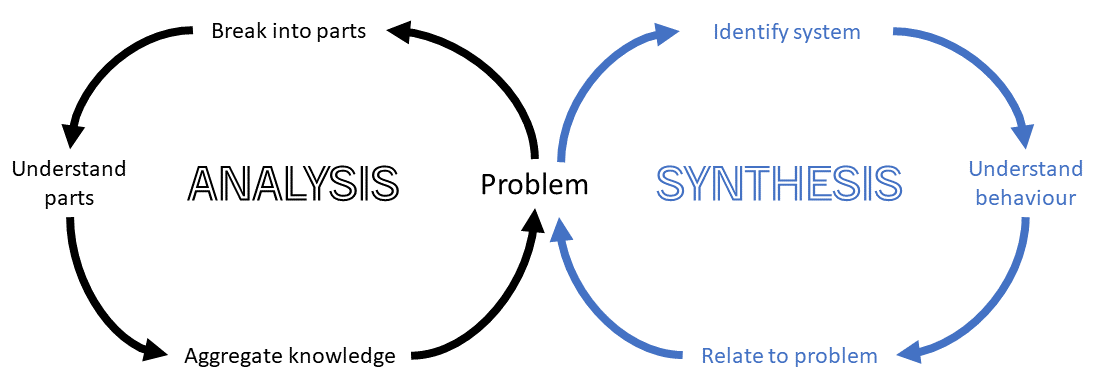
\includegraphics{./figures/Systems Thinking Defn Analysts.png}
	\caption[Why things happen][6pt]{Systems Thinking happens when you add Synthesis to Analysis Thinking. Synthesis seeks to explain why things happen, as opposed to analytical thinking, which focuses on constructing knowledge about what, when, where something is happening. The starting point for a systems inquiry is the question, what is this a part of? Understanding relationships that represent system causality allows for the further exploration of system behaviour.}
	\label{fig:stda}
\end{figure}

This approach is completely different to analytical thinking, because it does not seek understanding through a ‘reductionist scientific method’, but rather looks at challenges and problems as components of a wider system. This approach to problem solving seeks to understand the ‘whole system’ (cf. case study Appendices C, F and H). It is necessarily qualitative (or ‘soft’) when exploring what people think about the problem (often termed their hidden mental model).

System dynamics modelling, attempts to capture the developed shared-understanding of system structure in order to simulate the resulting dynamics of the system, potentially leading to greater knowledge about the system and enabling group learning. System modelling connects analytical thinking to the users of health intelligence in a useful way (cf. case study Appendices B, D, E, G). It allows them to explore the dynamics of quantitative knowledge in specific settings, eg. an ICS.

\subsection{Ackoff's definition of a 'system'}

Is it just something composed of other interrelated things, like your car, which is composed of parts: e.g. wheels, an engine, seats, a chassie, etc? Russel Ackoff liked to define a system in terms of the automobile, something most of us can relate to at some level. Who am I to argue with such a giant in the field of systems thinking?

An automobile is unlike any of its parts. You can drive a car. It carries you from one location to another and maybe some friends and your luggage/groceries/golf clubs or whatever you might be hauling about. That use or behaviour can't be found in any of the parts of a car. Only the car can carry you about. It is the system that moves you and stuff from place to place.

Your car has lots of parts, but from a systems point of view only some of them are essential parts of his system. However, even essential parts won't have an independent effect on the behaviour of the car. For example the engine provides the energy for motion, but is useless without the wheels to allow motion or a transmission and axels to connect the energy produced in the engine with the wheels. All of these essential parts have relationships with other parts, and are interdependent in terms of their effect on the system.

If, like me, you have taken your car apart to some extent (in an attempt at some repair undoubtedly), you will have noticed that your car was unable to perform its function in that state of disassembly. Its fundamental property, to move you and your stuff about the place, has disappeared. Therefore, while disassembled your car is no longer a system. It's just a lot of car parts cluttering your garage or driveway.

We only have a system (or indeed a car) when its behaviour differs from that of its parts. Although the systems we are interested in are predominately not mechanical, like cars, I find this to be a useful and far reaching analogy across all the systems of interest in public health practice:

\begin{itemize}[leftmargin=2cm]
	\item[organisms] systems with much greater complexity than your car, but the analogy holds and microbes, insect vectors, other animals of public health interest that might host pathogens or be hazardous in another way, and of course us (we are a special case due to this tricky concept called 'choice') are all composed of parts (most of which are essential) that depend on an interaction with at least one other part to to effect system behaviour
	\item[natural] systems are often separated into the major earth system components -- atmosphere, hydrosphere, geosphere, biosphere, and cryosphere, but ultimately there is only one earth system. We need to draw boundaries based on what problem we are trying to solve, therefore, we are often interested in parts of larger natural systems. Sometimes that might be a distinct ecosystems including soils and environmental microbiomes
	\item[social] systems include 'communities of people' (variously defined), organisations and what might be thought of as 'communities of organisations' defining healthcare, social care, or education systems for example (these can be tricky as the word 'system' is in common usage -- when you see it used as such ask yourself if it meets Ackoff's definition)
	\item[technical] systems of interest might include computing, transportation, utilities, essential public services, manufacturing and logistics -- their functioning impacts public health directly and indirectly by underpinning or influencing all other systems
\end{itemize} 

These 'types' of systems are offered to help you in your conceptualisation of systems, because most of the systems we are interested in are 'invisible' to those who are not looking. Donello Meadows famously said, "there is only one system", and because we can never deal with everything (think of the phrase 'boiling the ocean'), systems thinking requires us to conceptualise 'the system' in terms of the problem we are trying to solve.

%\section{Proactive Systems-Based Practice}
%\section{Think 'synthesis': Build proactive practice}
\section{Organisations also need to rethink their 'ways-of-working' and 'learning'}

Building a proactive public health means focussing on the structure and underlying worldviews that sustain our health problems. It consequently means moving away from our current near total focus on health events and their patterns.

\newthought{Current public health}: Through its intelligence and research functions, attempts to understand past health risk and outcomes in order to develop appropriate interventions that we hope reduces future risk and associated poor outcomes. Imagine driving your car on the motorway, with a completely blacked out windscreen. You are only able to anticipate traffic ahead by using your rear view mirror to watch the behaviour of traffic behind you, and near real time monitoring of the situation is only available by looking our your side windows. You cannot see further ahead than your side windows allow, so is it any surprise that you miss your exit and crash your car into the back of slower moving vehicles?

\newthought{Future public health}: Through its intelligence and research functions, creates accurate models of population health, and it uses these models to anticipate risks and outcomes before they occur, by understanding system behaviour. Imagine that you are on the same motorway in the same old car with a completely blacked out windscreen. Only now your car has two systems guiding it. System one is a self-driving capability that allows your car to know where it is at all times geographical and is able to sense cars immediately around it, enabling it to navigate to exits and to do this without crashing into other vehicles. System two provides a networked capacity to know what is happening throughout the road network so that it can anticipate and avoid the worst traffic. Just imagine.

%\section{Proactive public health practice transforms how we think about problems}
%\section{Systems-Based Problem Structuring}
%\section{Do system interventions: Manage problems}


Current analytical thinking practice is to deal with the problems we face one at a time, in isolation. To keep it simple. So we can understand it. Systems-based practice reframes identified problems into systems that contain the problem. The degree to which this facilitates successful management of the problem depends on how well we have identified the system containing the problem. A systems-aware public health practice is one that:
\begin{itemize}
	\item Moves from solving problems to managing problems
	\item Recognises that we face more than one 'type' of complexity
	\item Understands that shared-understand is a co-design process
	\item Understands that system intervention is a co-production process
\end{itemize}

\subsection{From solving to managing problems}
This is all about the structure of problems...

Ackoff has a lot to say on this subject matter -- managing the mess, also Theory of Constraints in the Goal, Checkland's soft systems work to develop shared-understanding on what problem we are trying to solve, etc.

\subsection*{Recognising complexity}

\subsection*{Shared-understand and co-design}

\subsection*{System intervention and co-production}




%\section{Transformative Systems-Based Public Health}
\section*{Learn together: Transform your organisation}

We talk a lot about transformation, transformative and transforming in public health and healthcare. Unfortunately, its mostly used simply as a synonym for 'change'. Or in some cases 'big change'. Transformation is defined as a change from one thing into something else. Anyone who's owned a kids toy called a Transformer, or seen the movies, knows what I'm talking about. Alien robots that transform into a completely different machine like cars, diggers or helicopters. Robot. Car. Not the same.

Systems-based public health can provide a transformative public health practice, because it:
\begin{itemize}
	\item Fundamentally shifts the way of working away from hierarchy and process into an Agile framework delivering co-design and co-production as a matter of course
	\item Humanises complex processes, relationships and organisations, which facilitates the changing of hidden mental models or worldviews
	\item Increases the scope of learning from individuals to organisations
\end{itemize}










This is a recounting of systems thinking that took place at Public Health Dorset, 2016-2020, a local public health system in South West England.

\subsection*{Mental models and co-design}
One of the fundamental aspects of synthesis thinking is that it can't be done in isolation -- unlike analysis thinking -- it requires as much perspective as possible. Synthesis thinking is literally 'team work'. It is defined by efforts to extract understanding from people. To share that understanding.

use of thinking tools

design thinking approach



\subsection*{System Dynamics Modelling}
Climate change model

Covid19 SEIR model


\subsection*{Preparing the future workforce}


\section{So now that we've seen the light, how do generate power?}
